%
\documentclass[aoas]{imsart}

%% Packages
\RequirePackage{amsthm,amsmath,amsfonts,amssymb}
\RequirePackage[authoryear]{natbib}
\RequirePackage[colorlinks,citecolor=blue,urlcolor=blue]{hyperref}
\RequirePackage{graphicx}
\RequirePackage{subfig}
\RequirePackage{multirow}
\RequirePackage{float}
\RequirePackage{url}
%----Helper code for dealing with external references----
% (by cyberSingularity at http://tex.stackexchange.com/a/69832/226)

\usepackage{xr}
\makeatletter

\newcommand*{\addFileDependency}[1]{% argument=file name and extension
\typeout{(#1)}% latexmk will find this if $recorder=0
% however, in that case, it will ignore #1 if it is a .aux or 
% .pdf file etc and it exists! If it doesn't exist, it will appear 
% in the list of dependents regardless)
%
% Write the following if you want it to appear in \listfiles 
% --- although not really necessary and latexmk doesn't use this
%
\@addtofilelist{#1}
%
% latexmk will find this message if #1 doesn't exist (yet)
\IfFileExists{#1}{}{\typeout{No file #1.}}
}\makeatother

\newcommand*{\myexternaldocument}[1]{%
\externaldocument{#1}%
\addFileDependency{#1.tex}%
\addFileDependency{#1.aux}%
}
%------------End of helper code--------------

% put all the external documents here!
\myexternaldocument{supplementary}

\startlocaldefs
%%%%%%%%%%%%%%%%%%%%%%%%%%%%%%%%%%%%%%%%%%%%%%
%%                                          %%
%% Uncomment next line to change            %%
%% the type of equation numbering           %%
%%                                          %%
%%%%%%%%%%%%%%%%%%%%%%%%%%%%%%%%%%%%%%%%%%%%%%
%\numberwithin{equation}{section}
%%%%%%%%%%%%%%%%%%%%%%%%%%%%%%%%%%%%%%%%%%%%%%
%%                                          %%
%% For Axiom, Claim, Corollary, Hypothesis, %%
%% Lemma, Theorem, Proposition              %%
%% use \theoremstyle{plain}                 %%
%%                                          %%
%%%%%%%%%%%%%%%%%%%%%%%%%%%%%%%%%%%%%%%%%%%%%%
\theoremstyle{plain}
\newtheorem{axiom}{Axiom}
\newtheorem{claim}[axiom]{Claim}
\newtheorem{theorem}{Theorem}[section]
\newtheorem{lemma}[theorem]{Lemma}
%%%%%%%%%%%%%%%%%%%%%%%%%%%%%%%%%%%%%%%%%%%%%%
%%                                          %%
%% For Assumption, Definition, Example,     %%
%% Notation, Property, Remark, Fact         %%
%% use \theoremstyle{remark}                %%
%%                                          %%
%%%%%%%%%%%%%%%%%%%%%%%%%%%%%%%%%%%%%%%%%%%%%%
\theoremstyle{remark}
\newtheorem{definition}[theorem]{Definition}
\newtheorem*{example}{Example}
\newtheorem*{fact}{Fact}
%%%%%%%%%%%%%%%%%%%%%%%%%%%%%%%%%%%%%%%%%%%%%%
%% Please put your definitions here:        %%
%%%%%%%%%%%%%%%%%%%%%%%%%%%%%%%%%%%%%%%%%%%%%%

\endlocaldefs


\begin{document}

\begin{frontmatter}
\title{Dynamic Prediction of the Target Survival Time in Metastatic Solid Tumor Cancer Clinical Trials}
%\title{A sample article title with some additional note\thanksref{t1}}
\runtitle{Dynamic Prediction of Target Survival Time}
%\thankstext{T1}{A sample additional note to the title.}

\begin{aug}
%%%%%%%%%%%%%%%%%%%%%%%%%%%%%%%%%%%%%%%%%%%%%%%
%% Only one address is permitted per author. %%
%% Only division, organization and e-mail is %%
%% included in the address.                  %%
%% Additional information can be included in %%
%% the Acknowledgments section if necessary. %%
%% ORCID can be inserted by command:         %%
%% \orcid{0000-0000-0000-0000}               %%
%%%%%%%%%%%%%%%%%%%%%%%%%%%%%%%%%%%%%%%%%%%%%%%
\author[A]{\fnms{Sidi}~\snm{Wang} \thanks{[\textbf{Corresponding author indication should be put in the Acknowledgment section if necessary.}]}\ead[label=e1]{sidiwang@umich.edu}\orcid{0000-0003-4838-0842}},
\author[A]{\fnms{Kelley}~\snm{Kidwell}\ead[label=e2]{kidwell@umich.edu}\orcid{0000-0002-1717-4483}},
\author[B]{\fnms{Bo}~\snm{Huang}\ead[label=e3]{Bo.Huang@pfizer.com}\orcid{0000-0002-3088-9328}}
\and
\author[B]{\fnms{Satrajit}~\snm{Roychoudhury}\ead[label=e4]{Satrajit.Roychoudhury@pfizer.com}\orcid{0000-0003-4001-3036}}
%%%%%%%%%%%%%%%%%%%%%%%%%%%%%%%%%%%%%%%%%%%%%%
%% Addresses                                %%
%%%%%%%%%%%%%%%%%%%%%%%%%%%%%%%%%%%%%%%%%%%%%%
\address[A]{University of Michigan, Department of Biostatistics \textbf{}\printead[presep={ ,\ }]{e1,e2}}

\address[B]{Pfizer Inc.\textbf{}\printead[presep={,\ }]{e3,e4}}
\end{aug}

\begin{abstract}
Overall survival (OS) is the gold standard for assessing patient benefit and cost-effectiveness of new cancer drugs. However, it is often difficult to use OS as the primary endpoint in randomized clinical trials (RCTs) for patients with metastatic cancer due to multiple reasons. In recent years, progression-free survival (PFS) has increasingly been used as the primary endpoint in metastatic cancer RCTs to accelerate development. However, regulatory authorities often seek mature OS data for approval. Therefore, it is critical to determine the target time when OS data are expected to be mature for reliable statistical inference. Motivated by an advanced renal cell carcinoma (RCC) clinical trial, we develop and investigate different prediction models leveraging information from disease progression to improve target OS prediction times. We propose a multivariate joint modeling approach considering components of progression and OS and extend two models commonly used for association to be used for OS prediction. To the best of our knowledge, this is the first comprehensive statistical study exploring the prediction of OS using different levels of information on disease progression and illustrating these models using a real, complex dataset. Our findings have significant implications for OS prediction.
\end{abstract}

\begin{keyword}
\kwd{Bayesian statistics}
\kwd{Multivariate joint modeling}
\kwd{Overall survival}
\kwd{Progression-free survival}
\kwd{Survival analysis}
\end{keyword}

\end{frontmatter}
%%%%%%%%%%%%%%%%%%%%%%%%%%%%%%%%%%%%%%%%%%%%%%
%% Please use \tableofcontents for articles %%
%% with 50 pages and more                   %%
%%%%%%%%%%%%%%%%%%%%%%%%%%%%%%%%%%%%%%%%%%%%%%
%\tableofcontents

\section{Introduction}

In recent years, many cancer drugs have received regulatory approvals based on results from phase 3 randomized clinical trials (RCTs) with progression-free survival (PFS) as the primary endpoint. Though PFS is well accepted as an intermediate endpoint for many cancer types, improvement in overall survival (OS) remains the clinical gold standard for assessing patient benefit \citep{tang2007surrogate, driscoll2009overall, methy2010surrogate, grigore2020surrogate} and cost-effectiveness \citep{royle2023overall} of a new drug. Planning a statistically well-powered OS analysis in practice is often challenging due to patients switching to alternative treatments after progression, non-response to treatment, starting other anti-cancer therapies, or being lost to follow-up. The timing of the RCT primary analysis with PFS as the endpoint is primarily driven by the number of patients who progressed. Therefore, at the time of the primary analysis, OS data are often not mature enough for meaningful statistical inference regarding treatment effects due to a low number of deaths. If PFS is statistically significant in the final analysis, regulatory agencies often request one or more updated OS analyses once the survival data are more mature. Thus, proper planning is necessary to understand when mature OS data will be available.
 
Model-based prediction of OS time for trial participants helps research teams allocate resources efficiently, plan future OS analyses accurately, and assess the likelihood of demonstrating the survival benefit of an experimental drug in the analysis. Accurate OS predictions not only facilitate the effective use of limited healthcare resources but also may benefit the patient in allowing the patient, their clinician, and family to make suitable plans for the remainder of the patient's life \citep{mackillop1997measuring}. \cite{sborov2019impact} demonstrated that when oncologists inaccurately predict OS, patients with advanced cancer are more likely to receive aggressive end-of-life care, which often contradicts the patients' wishes. 

Beyond drug approval and patient benefit, accurate OS predictions play a key role in determining the cost-effectiveness of a new drug and whether it is recommended for use in standard of care and reimbursement. Cost-effectiveness evaluations of new cancer treatments in health technology assessments rely on model-based extrapolation \citep{dias2011nice, latimer2011nice}. Various national health authorities, including the National Institute for Health and Care Excellence (NICE), the Pharmaceutical Benefits Advisory Committee, and the Canadian Agency for Drugs and Technologies in Health, provide guidance on appropriate extrapolation techniques for individual trials using parametric and semi-parametric distributions \citep{canadian2006guidelines, latimer2011nice, pharmaceutical2016guidelines}. \cite{heeg2022novel} have discussed a pragmatic two-step approach to select the optimal model and its corresponding distribution to ensure that the most plausible settings are being used for health technology assessment submissions. \cite{henderson2001accuracy} further provide examples of how accurate survival predictions have financial implications for insurance programs and health authorities. However, none of these approaches explored the relationship between progression and death to improve prediction accuracy.

When PFS is used as the primary endpoint, it captures the process of progression across target, non-target, and new lesions and death. That is, PFS is a composite endpoint defined as the time from randomization until progressive disease (PD) or death from any cause. In solid tumor studies, PD is evaluated using the Response Evaluation Criteria in Solid Tumors \citep{eisenhauer2009new}, commonly referred to as RECIST. The following four components comprise PFS: 1) measurement of the target lesion, which is captured as longitudinal continuous data; 2) time to worsening of the non-target lesion; 3) time to the emergence of a new lesion; and 4) time to death from any cause. Depending on the cancer type, each of these components has a different predictive degree of OS. For example, \cite{stein2013survival} showed that in Metastatic Renal Cell Carcinoma (RCC) the worsening of a non-target lesion or the appearance of a new lesion are more predictive of OS benefit than the sum of the longest tumor diameter of the target lesion. The current practice of OS prediction often ignores the disease progression process and models only the number of deaths.

In this manuscript, we develop and evaluate several model-based approaches to forecast the survival (death) times of trial participants ``still alive" leveraging information about disease progression and important baseline factors. Quantifying the relationship between disease progression and survival has garnered interest in both statistical and clinical literature over time. Among some of the notable ones, \cite{fleischer2009statistical} employed exponential time-to-event distributions to describe the dependency structure between OS and PFS. This is further expanded by \cite{fu2013joint, weber2019quantifying} and \cite{meller2019joint} by utilizing copula and multi-state models to jointly analyze PFS and OS without a strict parametric assumption for the marginal survival distributions of PFS and OS. \cite{shukuya2016relationship} investigated the correlation between median PFS and median OS, concluding that both tumor response and PFS are significant predictors of OS. Other methodologies for OS prediction include joint modeling of the longitudinal tumor size data of target tumor and survival data (\cite{claret2009model, claret2013evaluation, wang2009elucidation, bruno2014evaluation, zecchin2016models}, and \cite{lim2019predicting}). Meanwhile, \cite{yu2020new} jointly modeled the dynamics of target lesions and the progression of non-target lesions to predict PFS. However, most of the literature in this area are primarily focused on improving the estimation of OS rather than predicting the future survival time of patients ongoing in the trial. 

To our current knowledge, there is no existing method that formally combines all three components of disease progression along with additional uncertainties associated with death while predicting survival. We propose a multivariate joint modeling approach in this paper to fill that gap. Further, popular methods to analyze PFS and OS jointly, like the copula and multi-state model methods, have not previously been developed and illustrated for OS prediction. Hence, we extend the copula and multi-state models used primarily for association to be used for OS prediction. We compare OS predictions across these three novel methods and to a traditional marginal Weibull baseline hazard model of OS.

\section{Motivating Example: Phase 3 Study in Renal Cell Carcinoma} \label{sec:example}
The methods outlined in this paper are inspired by a phase 3, randomized, open-label, parallel-arm clinical trial \citep{motzer2019avelumab}. Treatment-naive adult participants with advanced RCC were randomized (1:1) to receive either the experimental drug or the active comparator, which was the standard of care. A key inclusion criterion was the presence of at least one measurable lesion, as defined by RECIST version 1.1. Tumor assessments were performed using computed tomography or magnetic resonance imaging at baseline, every six weeks post-randomization for the first 18 months, and subsequently every 12 weeks until confirmed disease progression. Important baseline demographic and disease characteristics were evenly distributed between the two treatment groups. The study had two primary endpoints: PFS and OS. The primary analysis was scheduled when at least 397 PFS events occurred (Figure \ref{fig:evolution}). At the time of the primary PFS analysis, only 146 deaths were observed, which was immature to draw any reasonable conclusion about the OS benefit provided by the new drug. Therefore, an updated analysis of OS was planned after 341 deaths in the trial. The trial findings indicated that patients administered the experimental drug experienced a notably extended PFS compared to those given the active comparator. It is crucial to note that while we have utilized the data structure from a real-life trial, the actual values presented here are simulated based on published summary statistics, both for proprietary considerations and to ensure proper protection of patient data.

\begin{figure}
    \centering
    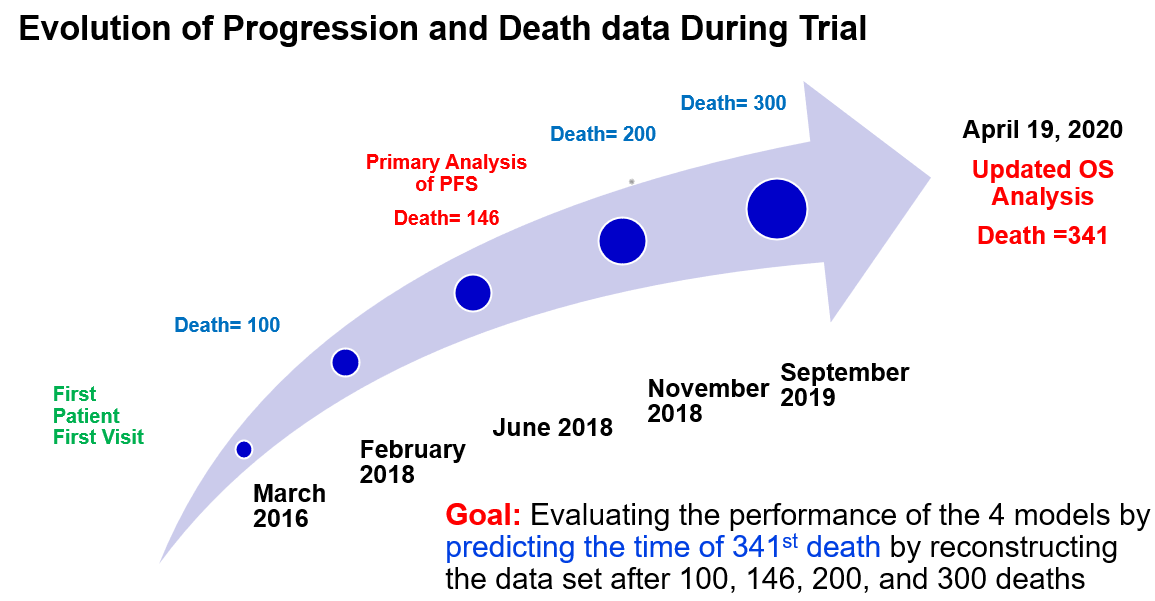
\includegraphics[width=0.85\textwidth]{img/Evolution.png}
    \caption{Evolution of progression and death data during trial\label{fig:evolution}}
\end{figure}


We aim to use the observed data to construct a predictive tool that reliably estimates the time of the $n$th death in the trial. In addition to timing, we are also interested in calculating the likelihood of demonstrating survival benefits in the updated OS analysis. This information is strategically and ethically important for retaining patients on the experimental drug. Specifically, we employ data on participants' baseline characteristics, treatment group, current survival status, and the details of tumor progression, i.e., target lesion measurements and the progression of disease of non-target and new lesions. We develop this model in the setting of RCC since PFS is known to be a good predictor of OS \citep{heng2011progression}, but the proposed model could be applied to other similar metastatic cancer settings.

Supplementary Figure \ref{fig:profile_LD} shows significant variability between individuals for the sum of the longest diameters of target lesions. Therefore, it is difficult to draw any conclusions about treatment without systematically modeling the variability. The Kaplan-Meier plots of non-target lesions and new lesions are shown in Supplementary Figure \ref{fig:NT_KMplot} and \ref{fig:NL_KMplot}. We observe a difference between the two treatment arms from both plots: patients who received the experimental drug had a longer time to PD considering non-target lesion and new lesion assessments. A similar trend is also observed in the Kaplan-Meier plots of OS (Supplementary Figure \ref{fig:OS_KMplot}) and PFS (Supplementary Figure \ref{fig:PFS_KMplot}). 

\section{Statistical Models for Milestone Prediction of Survival Endpoints}
\label{sec:method}

We present three different methods (Sections \ref{sec:jm}, \ref{sec:method_copula}, and \ref{sec:multistate}) for predicting milestone survival times based on disease progression information. These models use the components of tumor progression in different formats (e.g., as each component separately or as a composite endpoint) along with the available death data to predict the time of death for the ongoing patients. To understand the efficiency gain from progression data, we have included a parametric model (Section \ref{sec:method_standard}) that uses death information marginally, ignoring progression status. 

\subsection{Prediction Model Based on Jointly Modeling Different Components of Disease Progression}
\label{sec:jm}
%\subsection{Bayesian Model-Averaged Joint Modeling Approach}

We start with a new multivariate joint modeling approach that models the association between each component of disease progression and survival. Three separate models considering the association between survival and i) the sum of the longest diameter of target lesions, ii) the time to non-target lesion PD, and iii) the time to new lesion PD are proposed to explain the underlying heterogeneity of tumor progression dynamics and prevent information loss. In addition, we include a marginal model of current OS to take into account other intercurrent events (e.g., cross-over of control patient to treatment arm after progression) that can potentially affect the long-term survival of patients. 

The proposed multivariate joint modeling approach provides real-time OS predictions from each trial participant ``still alive" in two steps. First, we derive four sets of intermediate predictions based on the four models by fully encapsulating the association between progression and death. In the second step, we consolidate the OS predictions from all four models simultaneously using Bayesian model averaging (BMA) \citep{hoeting1999bayesian}. The structure of the proposed multivariate joint modeling approach is illustrated in Figure \ref{fig:JM}. 

\begin{figure}
\centering
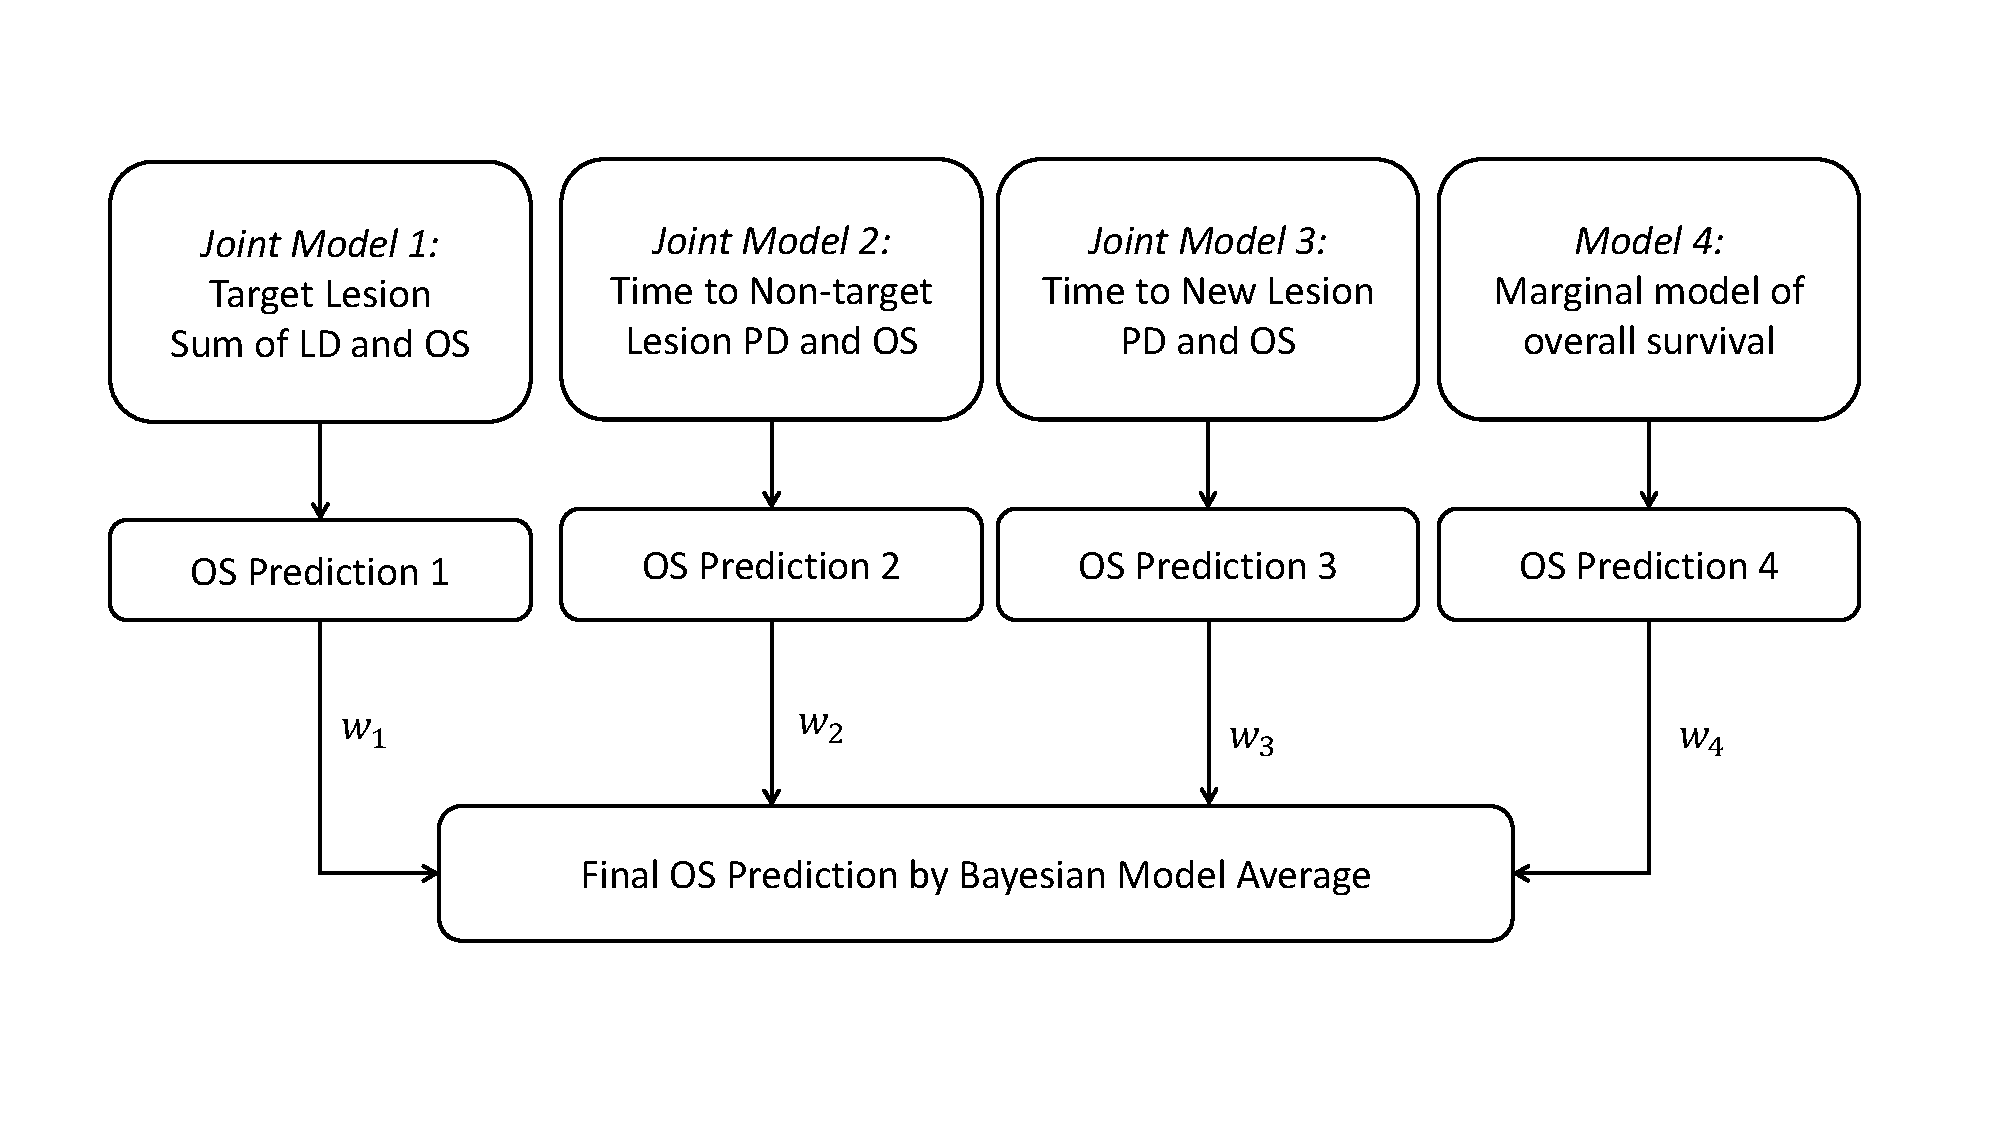
\includegraphics[width=\textwidth]{img/JM.pdf}
%\\
%\subfloat[]{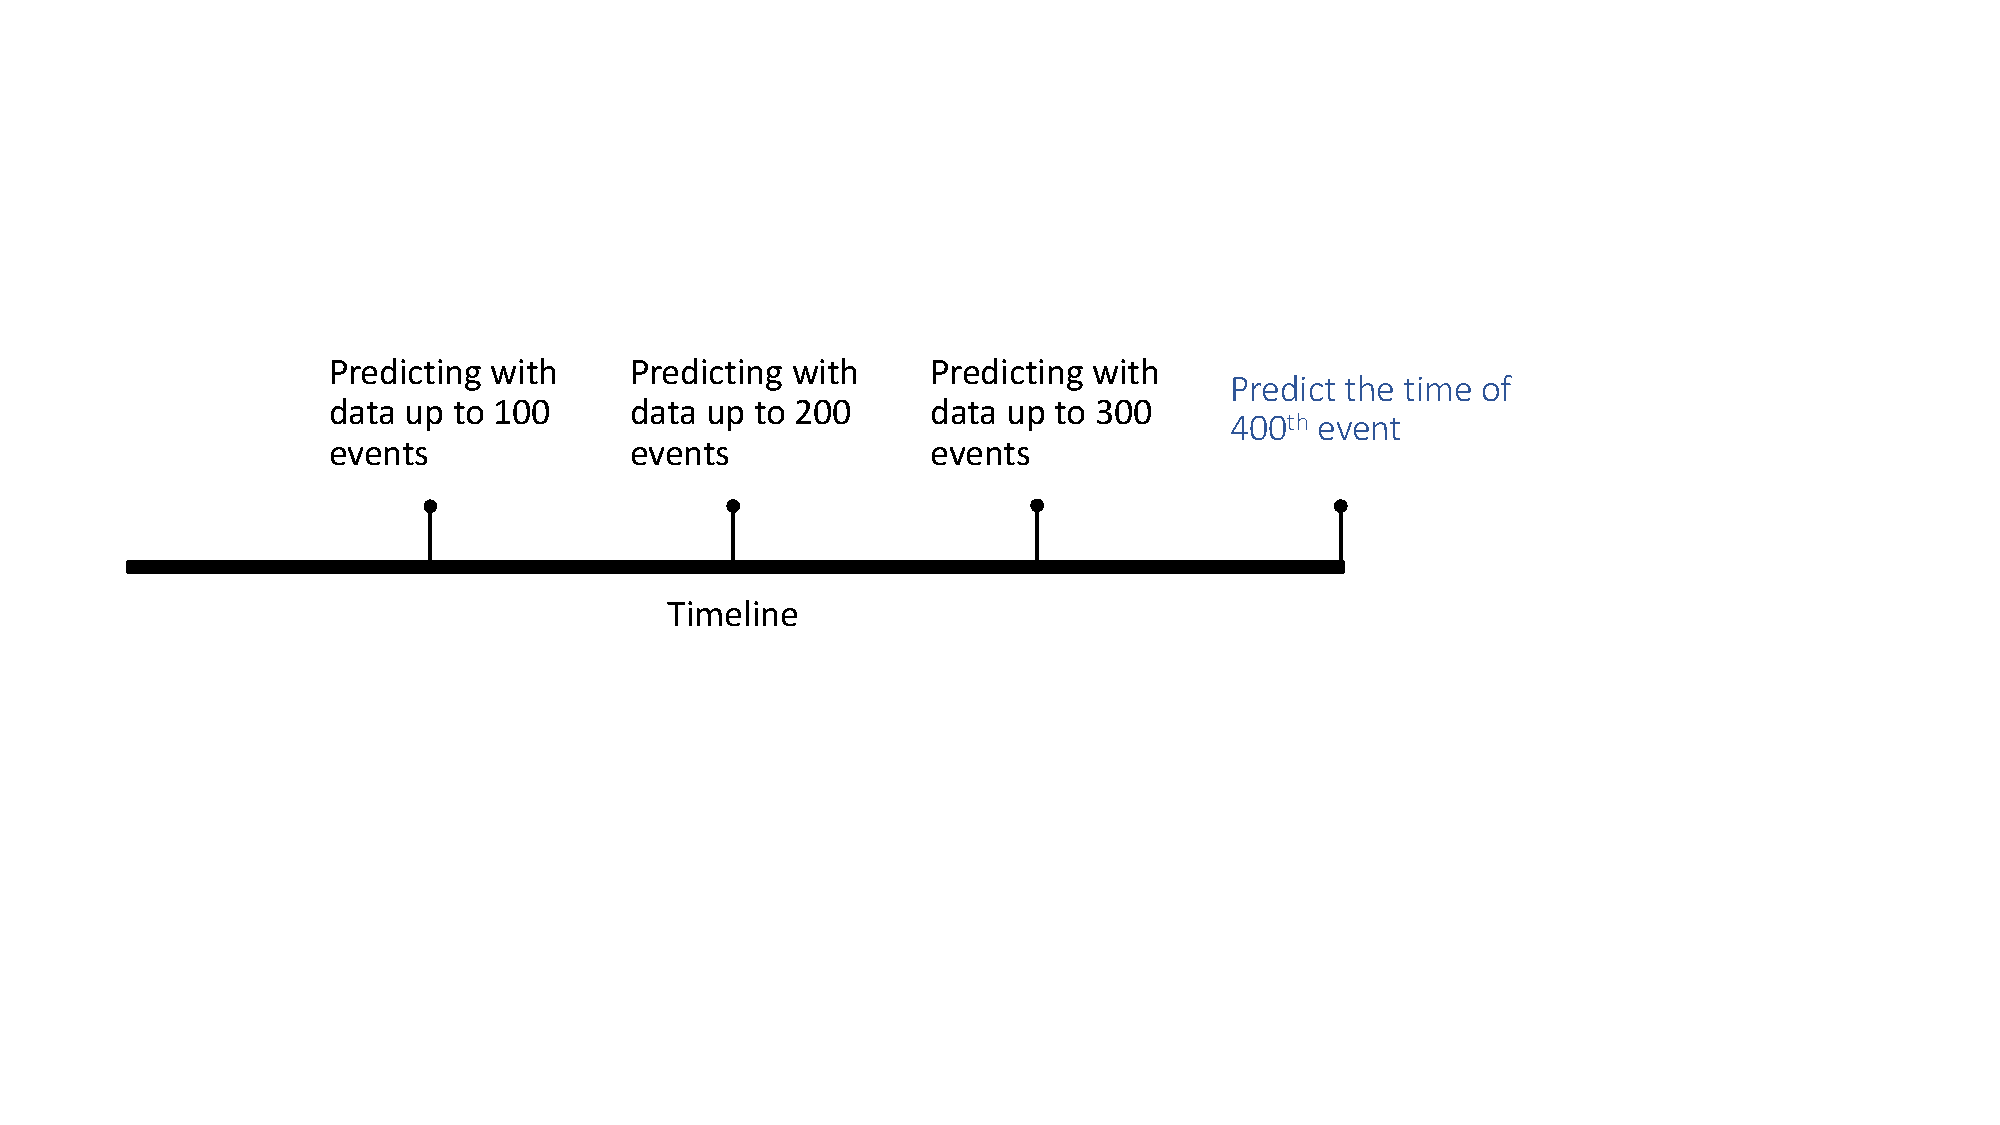
\includegraphics[width=\textwidth]{img/timeline.pdf}\label{fig:timeline}}
\caption{Multivariate joint modeling structure.} 
%(b) Predict the time of last (400th) event with observed data up to 100/200/300 events.}
\label{fig:JM}
\end{figure}


\subsubsection{Joint Model 1: the Association between Target Lesion and OS} \label{sec:TL}

A shared parameter model is used to explore the association between target lesion measurements and OS. We consider a set of $n$ subjects followed over an interval of time [0,$\tau$]. Let $z_{ij}$ be the target lesion measurement (or \% change from baseline in the sum of the longest diameter of target lesions) at time $t_{ij}$ (for the $i$-th participant at the $j$-th visit) where $i=1,...,n$ and $j=1,...,k_i$. We assume the target lesion measurement time $t_{ij}$ is non-informative so that it is independent of the longitudinal measurement and event-time processes for OS. This is a reasonable assumption as the tumor assessment timings were often specified in the protocol before study starts. We define a latent zero-mean Gaussian process $W_i(t)$ for the $i$-th participant, independent of different participants. The following sub-models link the joint model of lesion measurements and OS:
\begin{eqnarray*}
Y_{i}(t) \sim N(\mu_{i}(t), \sigma^{2}_{\epsilon}),
\end{eqnarray*}
where $Y_{i}(t)$ and $\sigma_{\epsilon}$ are the target lesion measurement for subject $i$ at time $t$ and variability associated with it. Moreover, the lesion measurement process $\mu(t)$ is modeled by the linear model
\begin{eqnarray*}
\mu_{i}(t) &=& \textbf{X}_i(t)' \boldsymbol{\beta}_{\mu}+W_{i}(t), \\
W_{i}(t) &=& b_{1i}+b_{2i}.
\end{eqnarray*}
Here, $\textbf{X}_i(t)$ refers to a time-dependent covariate matrix for subject $i$'s lesion measurement. Finally, $W_i(t)$ is a Gaussian process with ($b_{1i},b_{2i}$) being zero-mean bivariate Gaussian variables with variances $\sigma_1^2$ and $\sigma_2^2$ respectively, and correlation coefficient $\rho$. 

The OS process at time $t$ is modeled by a Weibull model:
\begin{eqnarray*}
\lambda(t) &=& \lambda_0(t) \exp(\textbf{Z}_i' \boldsymbol{\beta}_{\rm OS}+\lambda \mu_{i}(t)+b_{3i})\\
 &=& \alpha_{\rm OS,TL} \gamma_{\rm OS} t^{\alpha_{\rm OS,TL}-1} \exp(\textbf{Z}_i' \boldsymbol{\beta}_{\rm OS}+\lambda \mu_{i}(t)+b_{3i}),
\end{eqnarray*}
where $\textbf{Z}_i$ is a covariate matrix for OS, $\gamma_{\rm OS}$ and $\alpha_{\rm OS,TL}$ are the scale and shape parameters
of the Weibull distribution, and $b_{3i}\sim N(0,{\sigma_3})^2$ are random effects orthogonal to the measurement process. 

\subsubsection{Joint Models 2 and 3: the Association Between OS and Time to Worsening of Non-Target Lesion or Time to Appearance of New Lesion} \label{sec:NT}

Based on RECIST 1.1, the detailed tumor measurements of non-target and new lesions are not available at each visit. For example, we only know the current status of the non-target lesion (stable/worsen/disappear) and the appearance of a new lesion (yes/no). Moreover, this information is only available until the date of progression. Therefore, we use the time to worsening of non-target lesion (or time to appearance of new lesion) for the prediction model. The association between time to worsening of non-target lesion or time to appearance of new lesion and OS are explored using separate bivariate distributions. We used a copula-based model to capture the dependence between these survival times. Copulas are commonly used for modeling the dependence between random variables. They are continuous multivariate cumulative distributions with each random variable following a uniform marginal distribution on the interval $[0, 1]$. Sklar's theorem states that any multivariate joint distribution can be written using univariate marginal distribution functions and a copula describing the variables' dependence structure \citep{sklar1959fonctions}. 

We propose a Clayton copula function  \citep{clayton1978model} to model dependencies between time to worsening of non-target lesion (or time to appearance of the new lesion) and OS. The proposed class of Archimedean copula can capture strong dependence in the left tail. The relationship between time to worsening of non-target lesion (NT) (or time to appearance of new lesion (NL)) and OS is captured by a single parameter $\eta_{NT}$ (or $\eta_{NL}$), a parameter that can be directly linked to Kendall's tau, effectively characterizing their dependence. In the subsequent paragraphs, we formally define the copula model between time to worsening of non-target lesion (or time to appearance of new lesion) and OS. The model can be specified as
\begin{eqnarray*}
S_1(t_{\rm NT},
t_{\rm OS}|\textbf{Z}) &=& \{S_{\rm NT}(t_{\rm NT}|\textbf{Z})^{-\eta_{\rm NT}}
+S_{\rm OS}(t_{\rm OS}|\textbf{Z})^{-\eta_{\rm NT}}-1\}^{-1/\eta_{\rm NT}},\\
S_2(t_{\rm NL},
t_{\rm OS}|\textbf{Z}) &=& \{S_{\rm NL}(t_{\rm NL}|\textbf{Z})^{-\eta_{\rm NL}}
+S_{\rm OS}(t_{\rm OS}|\textbf{Z})^{-\eta_{\rm NL}}-1\}^{-1/\eta_{\rm NL}}. 
\end{eqnarray*}
Here $t_{NT}$, $t_{NL}$, and $t_{OS}$ denote times to worsening of non-target lesion, time to appearance of new lesion, and time to death (OS), respectively. $\textbf{Z}$ denotes the set of potential disease modifiers or baseline covariates for the prediction model. $\eta_{\rm NT}, \eta_{\rm NL}>0$ measures the correlation between time to worsening of non-target lesion or time to appearance of new lesion and OS. A large value of $\eta_{\rm NT}$ or $\eta_{\rm NL}$ represents a high correlation. When $\eta_{\rm NT}$ or $\eta_{\rm NL}$ goes to 0, the correlation approaches 0, and when $\eta_{\rm NT}$ or $\eta_{\rm NL}$ goes to $\infty$, the correlation converges to 1. Moreover, marginal survival probabilities are calculated using proportional hazard models expressed as:
\begin{eqnarray*}
S_{\rm A}(t_{\rm iA}|\mathbf{Z_{i}}) &=& \mathrm{exp}(-\int_{0}^{t} \lambda_{\rm A}(t_{iA}|\mathbf{Z_{i}})), \;\; \mbox{A= NT, NL, OS; $i=1,...,n$}, \\
\lambda_{\rm A}(t_{iA}|\mathbf{Z_{i}}) &=& \lambda_{0, \rm A}(t_{iA})\mathrm{exp}(\mathbf{Z_{i}}' \boldsymbol{\beta_{\rm A}}),\\
\lambda_{0, \rm A}(t_{iA}) &=& \gamma_{\rm A} t_{A}^{\alpha_{\rm iA}}
\mathrm{exp}(\mathbf{Z_{i}}' \boldsymbol{\beta_{\rm A}} ), \\
\alpha_{\rm iA}&=&\alpha_{A} + b_{iA}.
\end{eqnarray*}
Here, we introduce random effects for the shape parameter of the Weibull model ($b_{iA}$) to take into account the additional heterogeneity in the patient population.

Note that the censoring mechanism is associated with the time to worsening of non-target lesions, time to appearance of new lesions, and OS. The details of the likelihood construction under each joint model and implementation are provided in supplemental materials. 

\subsubsection{Model 4: Marginal Model for OS}\label{sec:marginal}

Finally, we introduce a marginal OS model to account for the risk of death not explained by disease progression. This includes scenarios when patients die without any evidence of disease progression or a change in risk of death due to exposure to other anti-cancer treatments after progression. A Weibull regression model similar to the marginal OS models mentioned in previous sections is used in this context.

\subsubsection{Prediction: Posterior Predictive Distribution (PPD)} \label{sec:PPD}
For each of the models in Sections \ref{sec:TL} - \ref{sec:marginal}, we utilize the PPD technique \citep{gelman2014bayesian} to generate OS predictions. The PPD represents the distribution of potential unobserved values based on the observed values, and it follows this structure:
$$p(y_{pred}|y) = \int{p(y_{pred},\theta|y)d\theta} = \int{p(y_{pred}|\theta,y)p(\theta|y)d\theta} = \int{p(y_{pred}|\theta)p(\theta|y)d\theta}.$$
This formulation leverages the conditional independence between $y$ (observed data), $y_{pred}$ (unobserved data), and $\theta$ (parameters). The PPD can be understood as an average of conditional predictions over the posterior distribution of $\theta$. During the MCMC process, for each sampled $\theta$ from the posterior distribution, a corresponding $y_{pred}$ sample is obtained. 

To produce PPD samples for OS using the models presented in the previous sections, we used \texttt{JAGS} software \citep{plummer2017jags} along with the \texttt{rjags} package for implementation in the R environment.

\subsubsection{Bayesian Model Averaging (BMA)}
We propose a Bayesian Model Averaging (BMA) method to combine OS predictions from the four models described in Sections \ref{sec:TL} - \ref{sec:marginal}. In prognostic modeling, it is standard to generate predictions by selecting a single model based on certain metrics. In the context of oncology, different PFS components may be more correlated with OS under various tumor types or patient groups, thus offering more accurate OS predictions. Here, we use BMA to calculate the weighted average of the predicted OS under the three joint models and one marginal model for the OS defined above. The weights indicate the plausibility of each model being the most predictive model. We denote the models defined in Sections \ref{sec:TL}, \ref{sec:NT}, and \ref{sec:marginal} by $M_T$, $M_{NT}$, $M_{NL}$, and $M_{OS}$, respectively. Then by BMA, the final predicted probability of OS follows
\begin{eqnarray*}
P(Y_{pred}|Data)&=&P(Y_{pred.t}|M_T,Data)P(M_T|Data)\\
&+&P(Y_{pred.nt}|M_{NT},Data)P(M_{NT}|Data)\\
&+&P(Y_{pred.nl}|M_{NL},Data)P(M_{NL}|Data)\\
&+&P(Y_{pred.os}|M_{OS},Data)P(M_{OS}|Data),
\end{eqnarray*}
where $P(M_T|Data)$, $P(M_{NT}|Data)$, $P(M_{NL}|Data)$, and $P(M_{OS}|Data)$ are model weights. In general, if we have a total of $Q$ models, the model weight for model $q$ at the $t$th MCMC iteration is  
$$w^{(t)}_q=P(M_q|Data,\theta^{(t)})=\frac{P(M_q,Data,\theta^{(t)})}{P(Data,\theta^{(t)})} =\frac{P(Data|M_q,\theta^{(t)})P(\theta^{(t)}|M_q)P(M_q)}{P(Data,\theta^{(t)})},$$
where $\theta^{(t)} = (\theta_1^{(t)}, \theta_2^{(t)},...,\theta_Q^{(t)})$. If we set $P(\theta_h|M_h, Data)=g_h$, and $q \ne h$, then according to \cite{congdon2007model},
$$P(\theta^{(t)}|M_q)=P(\theta_q^{(t)}|M_q) \prod_{h=1,h\ne q}^Q P(\theta_h^{(t)}|M_q)=P(\theta_q^{(t)}|M_q) \prod_{h=1,h\ne q}^Q g_h.$$
Therefore, 
\begin{eqnarray*}
w^{(t)}_q&=&P(M_q|Data,\theta^{(t)})\\
&=&\frac{P(Data|M_q,\theta^{(t)}_q) P(\theta^{(t)}_q|M_q) \prod_{h=1,h\ne q}^Q g_h P(M_q)}{\sum_{k=1}^Q P(M_k,Data, \theta^{(t)})} \\
&=&\frac{P(Data|M_q,\theta^{(t)}) P(\theta_q^{(t)}|M_q) \prod_{h=1,h\ne q}^Q g_h P(M_q) }{\sum_{k=1}^Q P(Data|M_k,\theta^{(t)}) P(\theta_k^{(t)}|M_k) \prod_{h=1,h\ne k}^K g_h P(M_k)}.    
\end{eqnarray*}
Through the above formulae, we implement the BMA approach and calculate the final predicted OS. 


\subsection{Prediction Models Based on Disease Progression as a Composite Endpoint}

\subsubsection{Copula Models for TTP and OS}
%\subsection{Copula Model for Time-to-Progression (TTP) and OS} 
\label{sec:method_copula}
Modeling TTP is similar to modeling PFS, but TTP excludes deaths from any cause. If a patient dies without documented disease progression, their TTP is censored at the last follow-up. Similar to the model defined in  \ref{sec:NT}, we use $\lambda_{\rm TTP}(t|\textbf{Z})$ to
denote the hazard function for TTP. Under the Cox
proportional hazards model, we have $\lambda_{\rm TTP}(t|\textbf{Z})=\lambda_{0, \rm TTP}(t)\mathrm{exp}(\textbf{Z}' \boldsymbol{\beta_{\rm TTP}})$, and the corresponding survival function is given by
$S_{\rm TTP}(t|\textbf{Z})=\mathrm{exp}\{-\gamma_{\rm TTP} t^{\alpha_{\rm TTP}}
\mathrm{exp}(\textbf{Z}' \boldsymbol{\beta_{\rm TTP}} )\}$, such that $\gamma_{\rm TTP}$ and $\alpha_{\rm TTP}$ are the scale and shape parameters
of the Weibull distribution, respectively. The Clayton model between TTP and OS is specified as
\begin{equation*}
S_1(t_{\rm TTP},
t_{\rm OS}|\textbf{Z})=\{S_{\rm TTP}(t_{\rm TTP}|\textbf{Z})^{-\eta_{\rm TTP}}
+S_{\rm OS}(t_{\rm OS}|\textbf{Z})^{-\eta_{\rm TTP}}-1\}^{-1/\eta_{\rm TTP}}, 
\end{equation*}
where $\eta_{\rm TTP}>0$ measures the correlation. Figure \ref{fig:copula} illustrates the Clayton copula fitted between TTP and OS.
The likelihood derivation can be found in supplementary materials. OS predictions are obtained using the PPD method described in Section \ref{sec:PPD}.

\subsubsection{Multi-State Model} \label{sec:multistate}
A multi-state model is another common approach for modeling the event history of participants in clinical trials \citep{andersen2002multi, meira2009multi, putter2007tutorial}, but currently, no literature has covered survival time prediction based on a multi-state model. Among the various multi-state models, the one that finds the widest application is the three-state illness-death model, which includes a singular immediate state denoting ``illness" (Supplementary Figure \ref{fig:multistate}). In this paper, we employ the homogeneous semi-Markov assumption \citep{cox1977theory} for the multi-state model, which implies that the hazard of death after progression depends on the time since progression rather than time since randomization. Therefore, for every patient, we examine two distinct periods: the time between randomization and progression, and the duration from progression to death. Both of these intervals are treated as separate components and modeled individually. A third scenario occurs when a patient dies without experiencing progression.

For the multi-state model, transition probabilities represent the probabilities of transition from one state to another over a given time period. Here, we denote the transition probability as $P_{kl}(t_1, t_2)$ from time $t_1$ to $t_2$, where $k$, $l$ describes the state with $k \in {0, 1, 2}$ and $l \in {0, 1, 2}$. The expressions of the transition probabilities are given by \citep{meira2009multi}:
\begin{eqnarray*}
P_{00}(t_1, t_2) &=& S_0(t_2 - t_1) = exp{(-\prod_{01}(t_2 - t_1) - \prod_{02}(t_2 - t_1))},\\
P_{11}(t_1, t_2) &=& S_1(t_2 - t_1) = exp{(-\prod_{12}(t_2 - t_1))},\\
P_{12}(t_1, t_2) &=& S_1(t_2 - t_1) = \int_{t_1}^{t_2}P_{11}(t_1, u) \pi_{12}(u;\mathcal{F}_u)P_{22}(u, t_2)du,
\end{eqnarray*}
where $\prod_{kl}(t_1, t_2)=\int_{t_1}^{t_2}\pi_{kl}(t, \mathcal{F}_t)dt$ is the cumulative transition intensity between states $k$ and $l$, where $k \leq l$. If we consider the transition intensities $\pi_{kl}(t; \mathcal{F}_t)$ to follow Weibull distributions, they can be expressed as
$\pi_{01}(t)=\alpha\left(1/\gamma_{01}\right)^\alpha t^{\alpha - 1},$
$\pi_{02}(t)=\alpha\left(1/\gamma_{02}\right)^\alpha t^{\alpha - 1},$
and $\pi_{12}(s)=\alpha\left(1/\gamma_{12}\right)^\alpha s^{\alpha - 1},$
where $\gamma_{01}, \gamma_{02}$ and $\gamma_{03}$ are the scale parameters, $\alpha$ is the shape parameter, $t$ refers to time since randomization and $s$ refers to time since progression. $\gamma_{01}, \gamma_{02}$ and $\gamma_{03}$ for each patient are further defined as $\gamma_{01,i} = \Tilde{\gamma}_{01}exp(\boldsymbol{\beta}_{01}\boldsymbol{X}_i)$, $\gamma_{02,i} = \Tilde{\gamma}_{02}exp(\boldsymbol{\beta}_{02}\boldsymbol{X}_i)$, and $\gamma_{12,i} = \Tilde{\gamma}_{12}exp(\boldsymbol{\beta}_{12}\boldsymbol{X}_i)$, respectively, where $i \in N$, $\boldsymbol{X}_i$ is a vector of covariates, and $\boldsymbol{\beta}_{01}$, $\boldsymbol{\beta}_{02}$ and $\boldsymbol{\beta}_{12}$ are regression coefficients. $\Tilde{\gamma}_{01}$, $\Tilde{\gamma}_{02}$, and $\Tilde{\gamma}_{12}$ are the baseline hazards. To guarantee the convergence of MCMC, a uniform shape parameter $\alpha$ is employed for all three Weibull functions. The multi-state model's likelihood construction is provided in supplementary materials. OS predictions are obtained using the PPD method described in Section \ref{sec:PPD}.

\begin{figure}
\centering
\subfloat[]{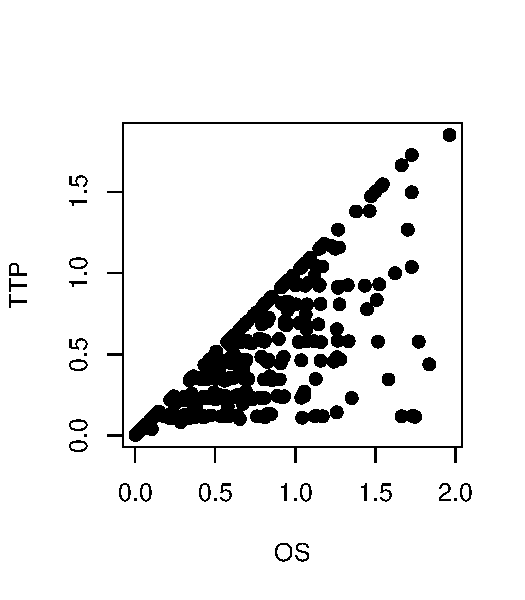
\includegraphics[width=0.31\textwidth]{img/scatterplot.pdf}}\label{fig:scatter}
\subfloat[]{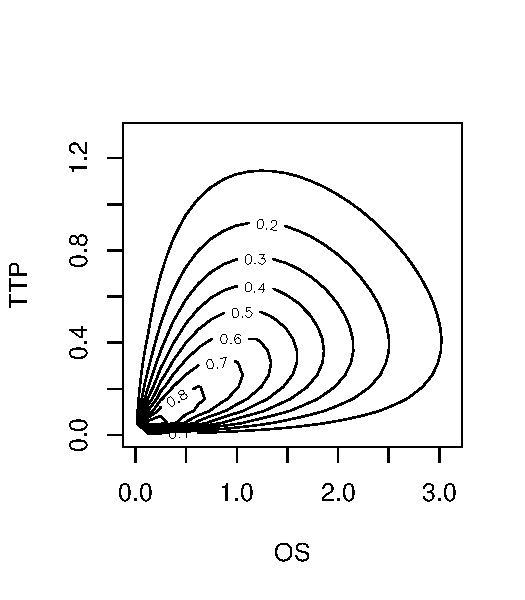
\includegraphics[width=0.325\textwidth]{img/contour.pdf}}\label{fig:contour}
\subfloat[]{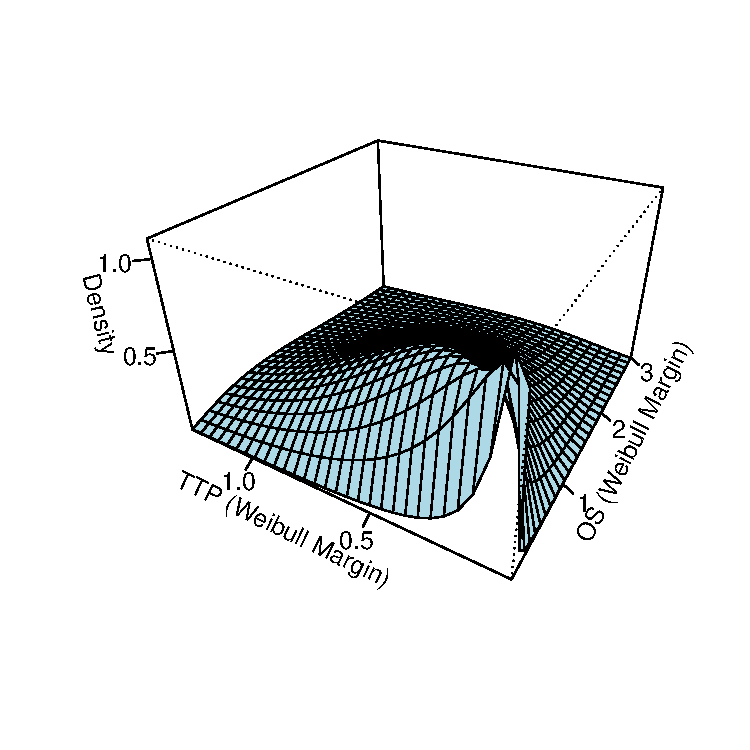
\includegraphics[width=0.35\textwidth]{img/surface.pdf}}\label{fig:surface}
\caption{(a) The scatterplot between time to progression (TTP) and overall survival (OS), (b) the contour plot of TTP vs. OS fitted with a Clayton copula, (c) the surface plot of TTP vs. OS fitted with a Clayton copula. \label{fig:copula}}
\end{figure}

\subsection{Marginal Weibull Baseline Hazard Model of OS}\label{sec:method_standard}

Most commonly, PFS is modeled using a Kaplan-Meier curve or Cox regression. For example, a simple Weibull baseline hazard model has the form
$\lambda(t)=\alpha \gamma t^{\alpha-1} \exp(\textbf{Z}' \boldsymbol{\beta})$,
where $\textbf{Z}_i$ is the covariate matrix for modeling PFS, $\alpha$ and $\gamma$ are the shape and scale parameters of the Weibull distribution, and $\boldsymbol{\beta}$ is a vector of coefficients. Note that a standard analytic method does not consider the dynamics of the component processes of PFS and does not take random effects into account.


\subsection{Prior Specification}

In this section, we provide recommendations for specifying priors for the parameters in the models discussed in Section \ref{sec:method}. Our aim is to promote the use of generalizable, weakly informative, or non-informative priors for all model parameters to ensure robust and interpretable results. We emphasize the importance of selecting appropriate priors to maintain parameter identifiability.

\subsubsection{General Guidelines}

For the $\boldsymbol{\beta}$ vector of coefficients, we recommend using weakly informative normal distributions with a mean of 0. We suggest weakly informative exponential distributions for the shape parameters ($\alpha$) in the Weibull distribution. All random effect parameters ($b$) should follow weakly informative normal distributions, denoted as $N(0, \sigma_{b_k}^2)$, where $k$ stands for different random variables under different models. Weakly informative half-normal priors are recommended for the standard deviations ($\sigma_{b_k}$) associated with the random effects. For all Clayton copula parameters ($\eta$), we recommend using weakly informative exponential distributions. These priors can accommodate a wide range of plausible values.

In the model assessing the association between target lesion and OS, which is a component of our proposed multivariate joint modeling approach, we suggest the following priors. For the parameter $\lambda$, a weakly informative normal distribution with a mean of 0 is recommended. The correlation coefficient ($\rho$) should have a non-informative prior, such as $Unif(-1, 1)$, to avoid biasing the estimation. Additionally, we assume that all models are equally weighted before fitting BMA, that is, $P(M_q) = 1/Q$, for all $q = 1,...,Q$.

In the multi-state model, we advise using weakly informative half-normal priors for all $\Tilde{\gamma}$ parameters. These priors allow flexibility while constraining extreme values.




\section{Simulations}
\label{sec:simulation}

\subsection{Design}
We performed extensive simulations to evaluate the performance of the proposed multivariate joint modeling approach. All simulated datasets mimic the structure of the RCC trial data. Specifically, we assume a trial with 400 subjects and 25 visits. Longitudinal measurements of target lesion and new lesion status are recorded at each visit. For simplicity purposes, non-target lesion status is not included. Survival status is updated whenever deaths occur. Follow-up visits occur every two months within the first two years, then change to every three months until the end of the fifth year. We censor the subject's subsequent target lesion measurements and new lesion status whenever that subject dies. 

We simulate under three scenarios: 1) OS is independent of both target lesion measurements and time to appearance of new lesion development; 2) OS is correlated solely with time to appearance of new lesion; and 3) OS is correlated only with target lesion measurements. In all scenarios, both target lesion measurements and new lesion statuses are simulated randomly and independently. However, OS is generated under varying conditions. Specifically, we simulate target lesion measurements using a linear mixed-effects model that incorporates time and treatment as fixed effects, alongside a patient-level random intercept and a random time effect. Furthermore, the time to appearance of new lesion is modeled using a Weibull baseline hazard function. In scenario 1, OS is randomly and independently simulated based on a Weibull baseline hazard function. In scenario 2, OS is conditionally simulated using a bivariate Clayton copula model, linking OS with time to appearance of new lesion. In scenario 3, OS is conditionally simulated based on target lesion measurements. Here, OS is still simulated using a Weibull baseline hazard function, but with an assumed negative correlation between quantiles of OS and larger tumor measurements. For each scenario, 100 datasets were generated. To streamline the simulation process, only treatment was included in the covariate matrices.

We compare predictions under four models: our proposed multivariate joint modeling approach, a copula model for TTP and OS, a multi-state model, and a marginal Weibull baseline hazard model of OS. 

\begin{figure}
\centering
\subfloat[]{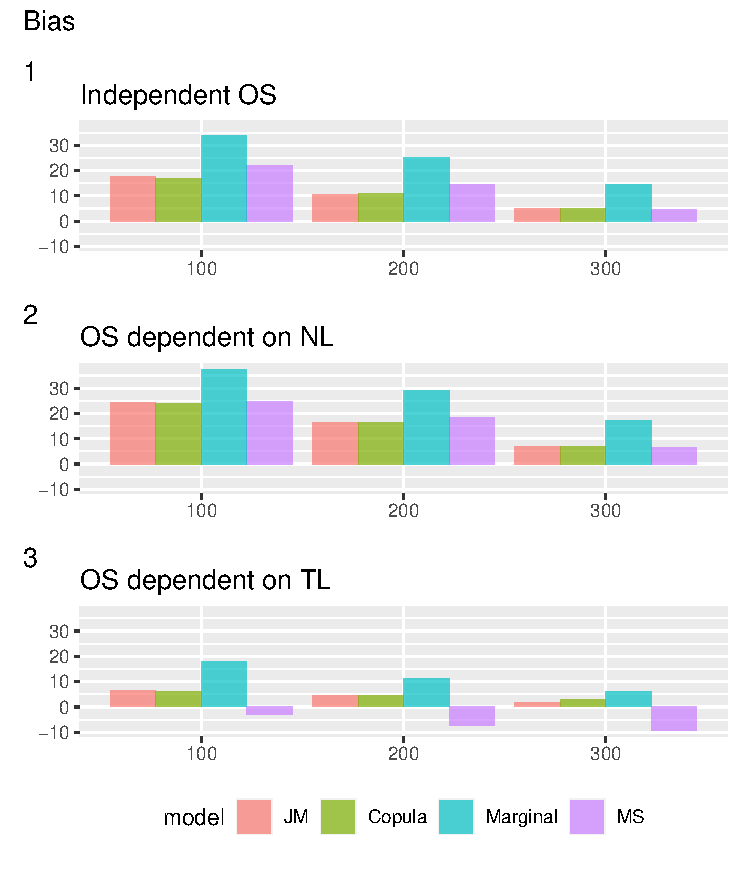
\includegraphics[width=0.5\textwidth]{img/Bias.pdf}\label{fig:bias}}
\subfloat[]{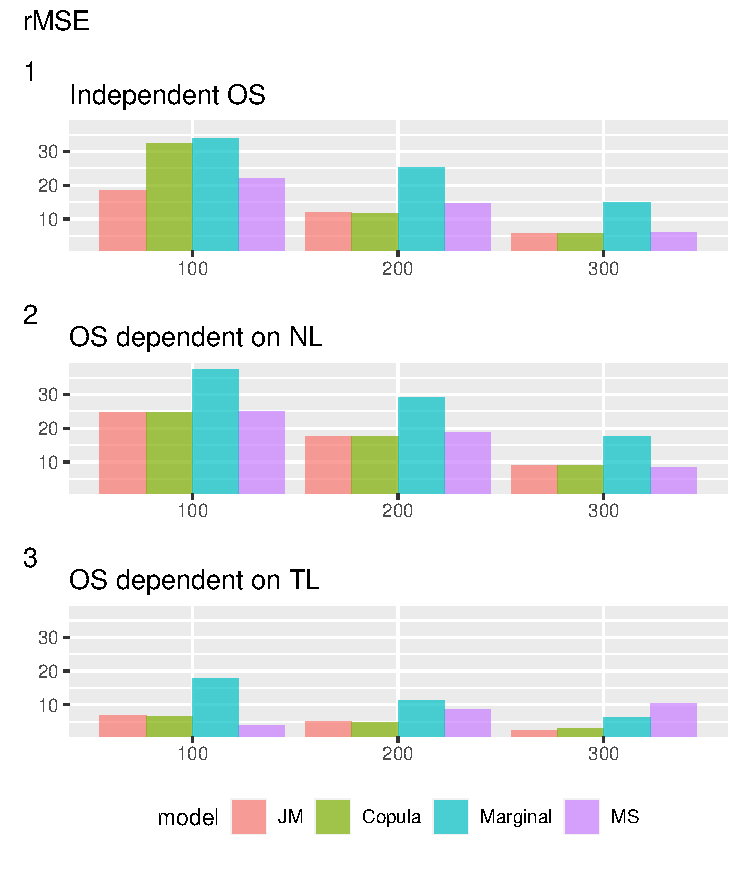
\includegraphics[width=0.5\textwidth]{img/rMSE.pdf}\label{fig:rmse}}
\caption{The bias (a) and root mean squared error (rMSE) (b) of the last (400th) death date predictors of four models: the multivariate joint modeling approach (JM), a copula model between TTP and OS (Copula), the marginal Weibull baseline hazard model of OS (Marginal), and a multi-state model (MS), under three OS scenarios. The $x$-axis denotes the number of deaths at the cutoff. The $y$-axis denotes the number of months. \label{fig:result}}
\end{figure}



To emulate real trial scenarios and assess the prediction performance of our proposed method, we generate snapshots of the data. For each simulated dataset, we took snapshots of what the data would have looked like if only 100, 200, and 300 death events had occurred. Then, we predicted the time of the last (400th) death event under each snapshot dataset. Note that predictions may be performed at any time during the trial, and 100, 200, and 300 were selected for illustration purposes. Predictions from the four methods were compared. Finally, we calculated each predictor's coverage rate (CR), root-mean-squared error (rMSE), bias, and width of the 90\% credible interval (CI). The 90\% CI is the narrowest interval that includes 90\% of the posterior distribution of the predictor. 

\subsection{Results}

The bias and rMSE of the predicted time of the last death are shown in Figures \ref{fig:bias} and \ref{fig:rmse}, and the corresponding CR and CI width are shown in Supplementary Table 1. The weights of all submodels of the multivariate joint modeling approach under each simulation scenario are shown in Supplementary Figure \ref{fig:weights_simulation}.

Under scenario 1, where OS is generated independently, the bias and rMSE of all predictors become smaller as we gather more information from the trial, i.e., more deaths are observed. Overall, the marginal model performs worse than the other three models. This is likely due to the Weibull model being conservative as it only utilizes OS data, causing predictions to concentrate near the observed maximum OS. Given that the proposed model assigned all the weight to the copula model between new lesion and OS, it is reasonable that the copula model and the multivariate joint modeling approach have similar bias and rMSE. Having evaluated all the metrics, the multivariate joint modeling approach and the copula model are the best-performing methods under scenario 1.

In scenario 2, where OS is generated based on new lesion status, the multivariate joint modeling approach, the copula model, and the multi-state model exhibit similar bias and rMSE values. Once again, the marginal model lags behind the other models in performance. As with scenario 1, as the number of observed deaths increases, the bias and rMSE of all predictors decrease. Compared to scenario 1, the improved performance in bias and rMSE of the multi-state model can largely be attributed to the fact that the OS observations generated under scenario 2 more closely resemble a Weibull distribution. However, when only 100 or 200 death events are observed, the multi-state model has a lower CR than the other two. This might be due to the standard Weibull model being a conservative model. Consequently, for scenario 2, we recommend either the multivariate joint modeling approach or the copula model.

In scenario 3, where OS is derived based on target lesion measurements, the proposed multivariate joint modeling approach begins to surpass the copula model as more deaths are observed. Simultaneously, as the count of observed deaths increases, the multivariate joint modeling approach assigns greater weight to the joint model between the target lesion and OS, which is anticipated. This is expected as the multivariate joint modeling approach is the only method that captures the relationship between OS and the target lesion. Differing from the other two scenarios, the bias and rMSE of predictors from the multi-state model do not consistently diminish with the increase in observed death events. Moreover, the multi-state model displays the widest CI among all the models. This can be attributed to the alteration in OS distributions, as it is generated based on the target lesion distribution, which does not conform to a Weibull distribution. The inflexibility of the standard Weibull baseline hazard model, devoid of random effects, further contributes to the wide intervals.

According to Figure \ref{fig:result}, across all scenarios, the proposed multivariate joint modeling approach performs either the best or very similar to the copula model, if the copula model performs best. This is reasonable as BMA could assign $w_q = 1$ to submodel $q$ when submodel $q$ is significantly better than the other $q-1$ submodels. If this is the case, the multivariate joint modeling approach predictions will be the same as the predictions from its submodel $q$. The multivariate joint modeling approach and the copula model are less sensitive to changes in the OS distribution and still provide relatively reasonable predictions even when OS prediction does not closely resemble a Weibull distribution. 

\begin{figure}
\centering
\subfloat[]
{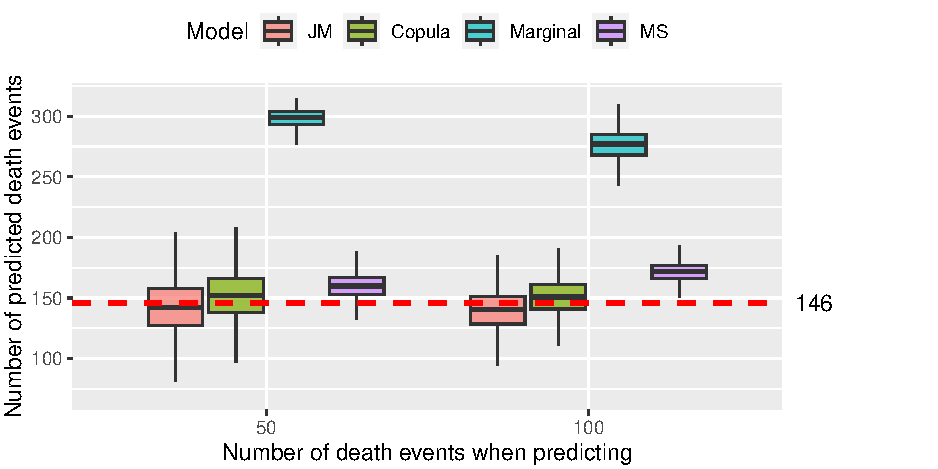
\includegraphics[width=0.75\textwidth]{img/primary_analysis.pdf}\label{fig:primaryanalysis}}
\hfill
\subfloat[]
{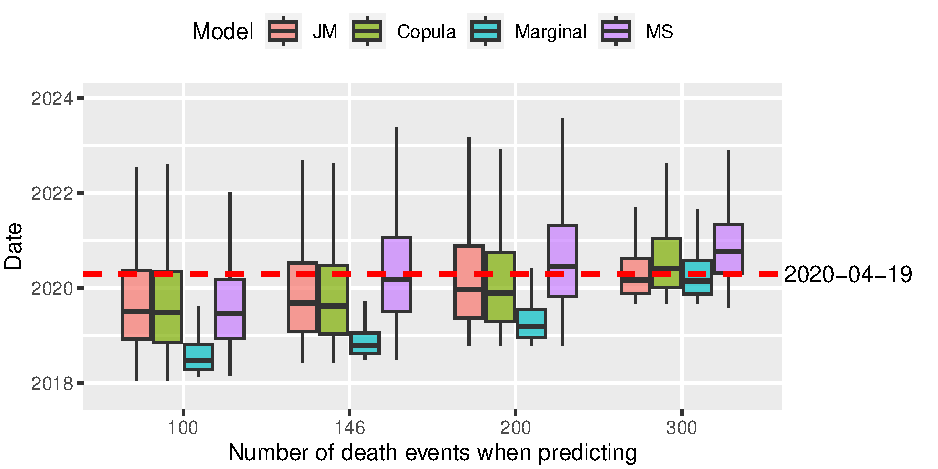
\includegraphics[width=0.75\textwidth]{img/lastdeath1.pdf}\label{fig:casestudy}}
\hfill
\subfloat[]
{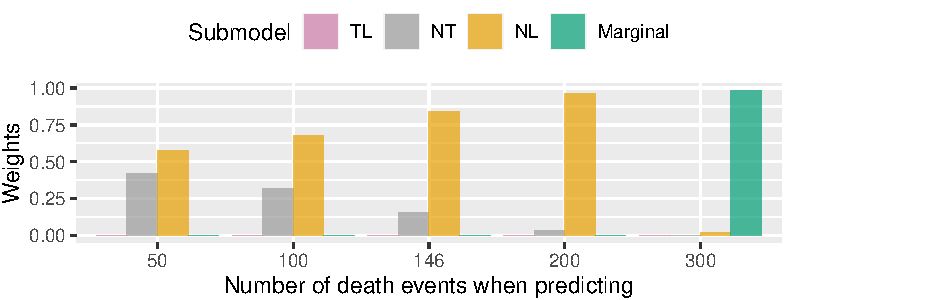
\includegraphics[width=0.75\textwidth]{img/weights.pdf}\label{fig:weights}}
\caption{\footnotesize (a) Boxplots of the predicted number of deaths at primary analysis when 50 or 100 deaths are observed in the trial, with the true number of deaths being ``146".(b) Boxplots of the posterior distributions of the last (341st) death date by the proposed multivariate joint modeling approach, the copula model between TTP and OS, the marginal Weibull baseline hazard model of OS, and the multi-state model. The date ``2020-04-19" is the true last (341st) death date. (c) The final weights of each submodel under the proposed multivariate joint modeling approach.}
\end{figure}

\section{Analysis of the Renal Cell Carcinoma Trial Data}
\label{sec:caseanalysis}
We return to the RCC trial dataset introduced in Section \ref{sec:example}. To evaluate the model's performance, we considered the trial data after 341 deaths were observed. The objective is to compare the predicted timing of the 341st death using different models described in Section \ref{sec:method} with the actual observed timing. The model's performance was further evaluated by comparing the number of deaths predicted by different models with the observed number of deaths at the PFS final analyses. For this exercise, we generated snapshots of the trial data at the 100th, 146th (the time of the primary analysis), 200th, and 300th death and compared predictions under four models: the multivariate joint modeling approach, a copula model for TTP and OS, a multi-state model, and a marginal model of OS. In addition to timing, we are interested in calculating the likelihood of demonstrating statistically significant OS in favor of the experimental drug at the updated OS analysis after 341 deaths.

We included \textit{gender, age, nephrectomy at baseline, Heng prognostic criteria at baseline, and ECOG Performance Status} into the covariate matrix $\textbf{X}_i$ and $\textbf{Z}_i$. Then, we fit each model using two MCMC chains, each with at least 10,000 MCMC iterations, in addition to 1,000 burn-in and 8,000 adaptation iterations. Convergence diagnostic tests, trace plots, and autocorrelation were investigated to ensure convergence (details provided in the supplementary materials). Figure \ref{fig:primaryanalysis} displays the predicted number of deaths at the time of the primary analysis. Figure \ref{fig:casestudy} presents boxplots of the predictive distributions for the predictors of the last (341st) death date from all tested models compared to the true last (341st) death date. The median values of the boxplots serve as point predictions. Figure \ref{fig:weights} displays the posterior weights of all submodels for each dataset based on the specified number of deaths. In this specific case study, the posterior odd favors the model explaining the correlation between new lesions and OS, which is aligned with the knowledge of the disease. The copula model between TTP and OS also performs well. While the marginal model exhibits significantly smaller CIs, its predictability has proven to be less accurate than those of the multivariate joint modeling approach and the copula model, especially after observing 100, 146, and 200 deaths. The performance of the marginal model improves consistently as the number of observed deaths increases. For example, the marginal model performs the best among all submodels after observing 300 deaths. The posterior weight from BMA favors the marginal model in this case and is reflected in Figures \ref{fig:casestudy} and \ref{fig:weights}. Considering that the posterior samples of the multi-state model are derived by combining predictions from two distinct time periods - randomization to progression and progression to death. Therefore,  it is reasonable for the multi-state model to exhibit the widest CIs. 

Table \ref{tab:casestudytable} presents the bias and rMSE of the predicted OS from different models when 100, 146, 200, or 300 death events are observed. In the first three scenarios, the multivariate joint modeling approach performs similarly to the copula model and the multi-state model. In the last scenario, the multivariate joint modeling approach performs similarly to the marginal model, consistent with the submodel weights shown in Figure \ref{fig:weights}. Additionally, the multivariate joint modeling approach exhibits smaller bias and rMSEs compared to the marginal model under all scenarios. While the multivariate joint modeling approach may not always have the smallest bias in this particular case study dataset, its prediction reliability is consistently verified. 

In addition, we calculated the likelihood of demonstrating statistically significant OS in favor of the experimental drug at the updated OS analysis (i.e., after observing 341 deaths), which is also included in Table \ref{tab:casestudytable} as the probability of success. The probability was calculated as the proportion of simulated trials in which the posterior probability of the underlying hazard ratio being less than 1 ($HR < 1$) exceeded 0.975. In this case study, the likelihood of demonstrating an OS benefit is high ($\geq 97\%$) due to the early trend of survival benefit. This high probability supports the retention of patients on the experimental drug.

Finally, We used four models to forecast the death time of patients who were still alive after 341 deaths were observed. Subsequently, we generated predicted Kaplan-Meier plots for each model (Figure \ref{fig:predictionKM}) and estimated the potential gain or loss in life expectancy by calculating the difference in the area under the curve between the experimental drug and the standard of care \citep{pak2017interpretability, survRM2}. The results from Figure \ref{fig:predictionKM} indicate that all models consistently project a substantial improvement in life years. In addition, the multivariate joint modeling approach and the copula model, whose reliability was previously established in this case study, both forecast a roughly 7.5-month gain in life years for patients who receive the experimental drug, as opposed to the standard of care.

\begin{table}
\caption{Bias, rMSE, and the probability of success (Prob) of the predictors of multivariate joint modeling approach (JM), copula model between TTP and OS, marginal model, and multi-state model (MS). \label{tab:casestudytable}}
\begin{center}
\begin{tabular}{ccccccc}
\hline
\multicolumn{2}{c}{No. of events} & \multirow{2}{*}{Metric} & \multirow{2}{*}{JM} & \multirow{2}{*}{Copula} & \multirow{2}{*}{Marginal} & \multirow{2}{*}{MS}\\ 
Observed & Predicted & & & & & \\\hline
\multirow{3}{*}{100} & \multirow{3}{*}{241} & Bias & 0.67 & 1.71 & 9.46 & 1.35\\
&& rMSE & 3.71 & 3.94 & 10.56 & 3.73 \\
&& Prob & 0.99 & 0.98 & 0.99 & 0.97 \\ \hline
\multirow{3}{*}{146} & \multirow{3}{*}{195} & Bias & 1.41 & 2.11 & 9.13 & 2.54\\
&& rMSE & 2.56 & 3.13 & 9.65 & 3.14 \\
&& Prob & 0.97 & 0.99 & 0.99 & 0.98 \\ \hline
\multirow{3}{*}{200} & \multirow{3}{*}{141} & Bias & 0.91 & 2.15 & 7.89 & 3.11\\
&& rMSE & 2.06 & 2.91 & 8.19 & 3.65 \\ 
&& Prob & 0.98 & 0.98 & 0.98 & 0.97 \\ \hline
\multirow{3}{*}{300} & \multirow{3}{*}{41} & Bias & 6.23 & 2.97 & 6.32 & 4.13  \\
&& rMSE & 8.24 & 6.14 & 8.28 & 7.31  \\ 
&& Prob & 0.97 & 0.97 & 0.97 & 0.97  \\ \hline
\end{tabular}
\end{center}
\end{table}



\begin{figure}
    \centering
    \subfloat[]{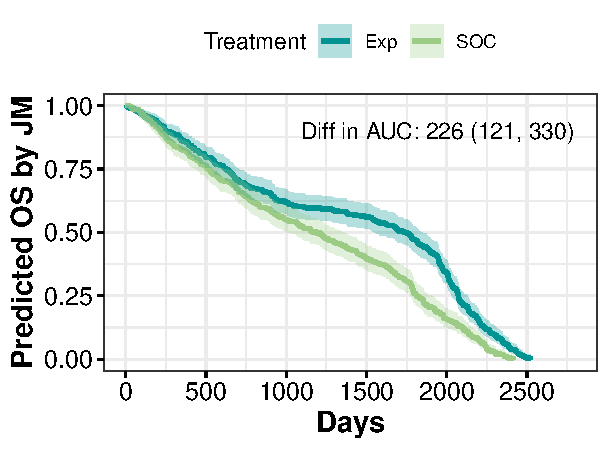
\includegraphics[width=0.49\textwidth]{img/JMprediction.pdf}}\label{fig:JMprediction}
    \subfloat[]
    {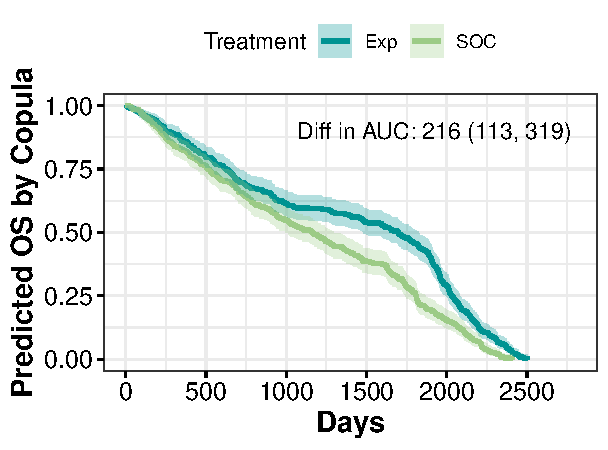
\includegraphics[width=0.49\textwidth]{img/copulaprediction.pdf}}\label{fig:Copulaprediction}
    \hfill
    \subfloat[]{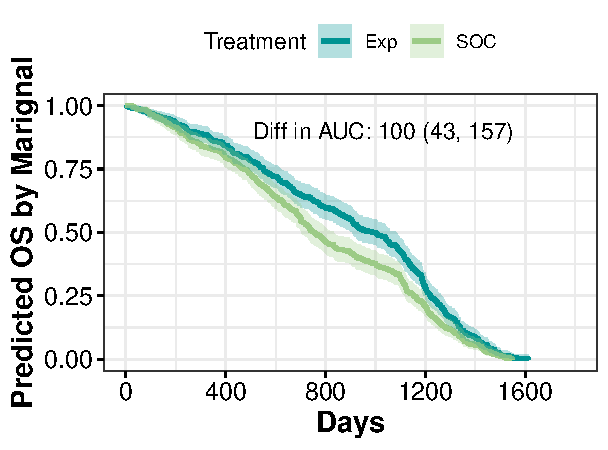
\includegraphics[width=0.49\textwidth]{img/marginalprediction.pdf}}\label{fig:Marginalprediction}
    \subfloat[]{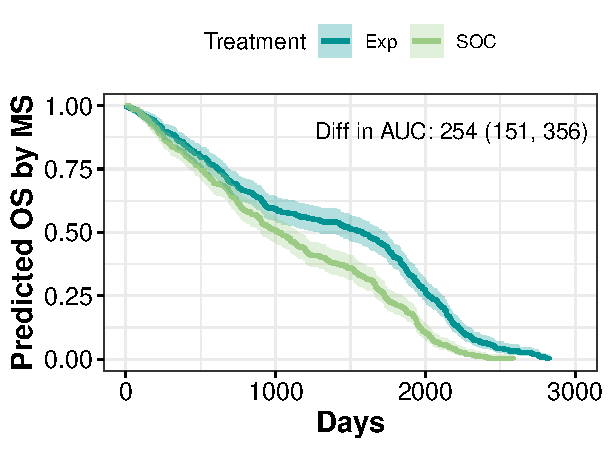
\includegraphics[width=0.49\textwidth]{img/MSprediction.pdf}}\label{fig:MSprediction}
    \caption{Kaplan-Meier plots of the observed and predicted overall survival by the multivariate joint modeling approach (a), the copula model (b), the marginal model (c), and the multi-state model (d). The difference in the area under the curve (AUC) and its credible intervals for the experimental drug (Exp) and the standard of care (SOC) are also included.}
    \label{fig:predictionKM}
\end{figure}

\section{Discussion}
\label{sec:discussion}
We were motivated by an advanced RCC clinical trial to present how real-time OS predictions from joint models with different components of PFS can be dynamically combined via BMA. This multivariate joint modeling approach provides reliable estimates of the time of the $n$th death and the likelihood of demonstrating OS benefit after observing $n$ deaths in a trial using all available tumor assessment data based on RECIST 1.1. This is valuable for clinical trial planning and patients' end-of-life medical care. Furthermore, the proposed multivariate joint model approach provides reliable and robust predictions in the case study and across all the scenarios we tested in the simulation studies. This approach can be applied to other solid tumor types beyond RCC.

The multivariate joint modeling approach is flexible and can easily incorporate a linear model with time-dependent covariates or a nonlinear mixed-effects model. Although Bayesian Model Averaging (BMA) methods optimally combine multiple models, they typically require extended training time due to their complexity. In the example data analysis, only five covariates were included. Incorporating additional baseline characteristics is possible, but doing so would expand the covariate matrix and further increase the computational demands of the multivariate joint modeling approach. Considering that the covariates utilized in each submodel may vary, it is beneficial to determine the most suitable covariates for each submodel before implementation. This covariate selection process can be guided by expert opinion or variable selection models, potentially reducing the size of the covariate matrix.

Based on the simulation studies and the example data analysis, it is evident that the copula model for TTP and OS ranks as the second most reliable model among all those tested. If the TTP and OS data are well-fitted by Weibull distributions with random effects, the copula model typically performs better than the marginal OS model. Therefore, fitting only a copula model with random effects is an excellent option to reduce model training time. Based on our simulations, without including random effects, high variability between individuals will cause the copula model's predictions to be too heavy-tailed.

For a marginal OS model to perform better, it would be beneficial to incorporate more predictive covariates or use a model offering greater flexibility than the Weibull baseline hazard model, such as piecewise exponential models. Similarly, to improve the performance of the multi-state model, we could replace the Weibull baseline hazard model with more flexible models.

During the simulation studies, the data for non-target lesions were not simulated, yet they were included in the example data analysis. This does not undermine the outcome of our simulation studies, given that both the non-target lesion and new lesion were modeled using the exact same joint model, and each component of PFS was modeled separately. If the non-target lesion data had been included in the simulation dataset, we would have anticipated longer training times for the multivariate joint modeling approach without observing any relative improvement in performance.

Apart from applying the same model weights for all the patients in the dataset, BMA can potentially provide personalized model weights, where each patient may have different weights for each model. This could further improve the prediction accuracy. Future work can explore how to implement personalized model weights in a time-efficient manner under the setting of this study.


%%%%%%%%%%%%%%%%%%%%%%%%%%%%%%%%%%%%%%%%%%%%%%
%% Funding information, if any,             %%
%% should be provided in the                %%
%% funding section.                         %%
%%%%%%%%%%%%%%%%%%%%%%%%%%%%%%%%%%%%%%%%%%%%%%


%%%%%%%%%%%%%%%%%%%%%%%%%%%%%%%%%%%%%%%%%%%%%%
%% Supplementary Material, including data   %%
%% sets and code, should be provided in     %%
%% {supplement} environment with title      %%
%% and short description. It cannot be      %%
%% available exclusively as external link.  %%
%% All Supplementary Material must be       %%
%% available to the reader on Project       %%
%% Euclid with the published article.       %%
%%%%%%%%%%%%%%%%%%%%%%%%%%%%%%%%%%%%%%%%%%%%%%
\begin{supplement}
\stitle{Title of Supplement A}
\sdescription{Short description of Supplement A.}
\end{supplement}
\begin{supplement}
\stitle{Title of Supplement B}
\sdescription{Short description of Supplement B.}
\end{supplement}

%%%%%%%%%%%%%%%%%%%%%%%%%%%%%%%%%%%%%%%%%%%%%%%%%%%%%%%%%%%%%
%%                  The Bibliography                       %%
%%                                                         %%
%%  imsart-nameyear.bst  will be used to                   %%
%%  create a .BBL file for submission.                     %%
%%                                                         %%
%%  Note that the displayed Bibliography will not          %%
%%  necessarily be rendered by Latex exactly as specified  %%
%%  in the online Instructions for Authors.                %%
%%                                                         %%
%%  MR numbers will be added by VTeX.                      %%
%%                                                         %%
%%  Use \cite{...} to cite references in text.             %%
%%                                                         %%
%%%%%%%%%%%%%%%%%%%%%%%%%%%%%%%%%%%%%%%%%%%%%%%%%%%%%%%%%%%%%

%% if your bibliography is in bibtex format, uncomment commands:
\bibliographystyle{imsart-nameyear} % Style BST file
\bibliography{reference}       % Bibliography file (usually '*.bib')


\end{document}
